\documentclass[oneside,12pt,openany]{book}
\usepackage[toc,page]{appendix}
\usepackage{amsmath,amsthm,amsfonts,indentfirst,graphicx,subcaption,textcomp,commath,mathtools,hyperref,pgfplots,epigraph,enumitem,pdfpages}

\hypersetup{
	colorlinks=true,
	linkcolor=blue,
	filecolor=blue,      
	urlcolor=blue,
	citecolor=blue,
	bookmarks=true,
}

\usepackage{scrextend}
\usepackage{afterpage}
\newcommand\blankpage{
	\vfill
	\pagebreak
	\ifthispageodd{\null
		\vfill
		\vfill
		\clearpage}{}
}

\renewcommand{\baselinestretch}{1.5}
\setlength{\textwidth}{6in}

\setlength{\oddsidemargin}{.5in} \setlength{\evensidemargin}{0mm}

\newtheorem{defn}{Definition}[section]
\newtheorem{thm}{Theorem}[section]
\newtheorem{lemma}{Lemma}[section]
\newtheorem{cor}{Corollary}[section]
\newtheorem{prop}{Proposition}[section]
\newtheorem{exa}{Example}[section]
\newtheorem{clm}{Claim}[section]
\newtheorem{rmk}{Remark}[section]
\newtheorem{case}{Case}[section]

\DeclarePairedDelimiter\ceil{\lceil}{\rceil}
\DeclarePairedDelimiter\floor{\lfloor}{\rfloor}
\newcommand{\rpm}{\raisebox{.2ex}{$\scriptstyle\pm$}}

\begin{document}
	\frontmatter
	\begin{titlepage}
		\centering
		{\scshape\Large \textbf{CAPTURING THE PREDICTIVE POWER OF CORTICAL LEARNING ALGORITHMS} \par}
		\vspace{5.5cm}
		{\scshape\large By \par}
		{\scshape\large Alexander C Michels\par}
		\vfill
		{\large Submitted to the Department of Computer Science and Mathematics\par}
		{\large Westminster College, New Wilmington, PA\par}
		{\large In partial fulfillment of the requirements for Honors Research\par}

		\vfill
		advised by\par
		\large
		Carolyn Cuff, Ph.D.\par
		C. David Shaffer, Ph.D.\par
		William Procasky, Ph.D.\par
		
		\vfill
		
		% Bottom of the page
		{\large \today\par}
	\end{titlepage}
	\renewcommand{\baselinestretch}{.7}
	\setcounter{tocdepth}{1}
	\tableofcontents
	\vfill
	\pagebreak
	
	\renewcommand{\baselinestretch}{1.5}
	
	\addcontentsline{toc}{chapter}{Acknowledements}
	\chaptermark{ACKNOWLEDGEMENTS}
	\begin{center}
		\textbf{ACKNOWLEDGEMENTS}
	\end{center}

	\textcolor{red}{Type your acknowledgements here}
	\vfill
	\pagebreak
	
	\addcontentsline{toc}{chapter}{Abstract}
	\chaptermark{ABSTRACT}
	\begin{center}
		\textbf{ABSTRACT}
		
		\begin{quotation}
			\noindent Hierarchical Temporal Memory (HTM) is model of intelligence based on the the interactions of pyramidal neurons in the mammalian neocortex currently being developed by Numenta. It has stood out from other machine learning techniques due to high noise tolerance and learning capacity making it well-suited for anomaly detection, prediction, signal processing, and sensorimotor processes. We seek to find a mathematical analogy to the predictive power of this biologically constrained theory using models from time series analysis. To do this, we statistically analyzed the error in predictions of HTM networks that we asked to predict outputs of autoregressive integrated moving average (ARIMA) models, varying the parameters of both the networks and the ARIMA models. We hope to to find a relation between sets of HTM network parameters and ARIMA model parameters to better explain the functions of each part of the neocortex and cortical learning algorithms in sequence memory.
		\end{quotation}
		
	\end{center}
	\vfill
	\pagebreak
	
	\addcontentsline{toc}{chapter}{List of Figures}
	\chaptermark{LIST OF FIGURES}
	\listoffigures
	\vfill
	\pagebreak
	
	\chaptermark{LIST OF TABLES}
	\listoftables
	\addcontentsline{toc}{chapter}{List of Tables}
	\vfill
	\pagebreak
	
	
	\begin{center}
		\textbf{\LARGE CHANGE LOG}
	\end{center}
	\begin{itemize}
		\item Brought over Chapter 1 from Proposal with edits and will add an ``Evolutionary Computing'' section to segue into HTM
		\item Brought over Sparse Distributed Representations from Proposal (Section 3.2) 
		\item Wrote some of ``Hardware and Software Specifications'' (Section 5.1)
		\item Wrote some on Swarming (Section 5.2)
	\end{itemize}
	
	
	\vfill
	\pagebreak
	
	\mainmatter
	\chapter{Introduction}
	
	Although we are continually bombarded with sensationalist news stories proclaiming the dawn and dangers of ``artificial intelligence,'' it is important to first define what it means to say a machine is intelligent. This is much the same way Turing began his preponderance of artificial intelligence in his 1950 \textit{Computing Machinery and Intelligence} \cite{Turing}. Turing came up with an eloquent boundary for determining the point at which we call a machine `intelligent.' His proposal, which he called ``The Imitation Game,'' but is now referred to as ``The Turing Test,'' is to have an interrogator question a human and an artificial intelligence, randomly labeled X and Y, in the hopes of distinguishing between the two \cite{Turing}. We reach ``intelligence'' when an interrogator cannot reliably distinguish between the two \cite{Turing}.
	
	As mathematicians, we could also take our favorite route of defining something: we look at a collection of things that we would agree to be ``intelligent'' and abstract the shared properties we consider to be desirable until we have a set of properties that must be met for a system to be considered intelligent. From this approach, we could say that a system \textbf{S} is intelligent if and only if it is able to ``use language, form abstractions and concepts, solves kinds of problems now reserved for humans, and improve themselves'' \cite{Jones}. This is the definition from the Dartmouth AI Summer Research Project, but such a definition is obviously hard to evaluate and it would be much more difficult to form a consensus on what set of properties define intelligence than it is to get a set of properties to define other abstract mathematical concepts such as an integral domain.
	
	It quickly becomes apparent that we also need more states than just the two Boolean ``intelligent''/``not intelligent'' ones to talk about intelligence in a constructive manner. Without this everything on the spectrum from a for loop with an if-else to the robots in Isaac Asimov's \textit{I, Robot}  are under the same label of ``not intelligent'' yet we know that the `intelligence' exhibited in those cases are not at all comparable. We need a spectrum with many states of intelligence to constructively talk about the intelligence of a system.
	
	John Searle's 1980 paper ``Minds, Brains, and Programs'' introduced the world to The Chinese room argument \cite{Searle}. It supposes that artificial intelligence research is successful and produces an artificial intelligence that is capable of behaving as if it understands Chinese, then asks does the machine literally understand Chinese or it simulating the ability to understand Chinese \cite{Searle}? Although this may seem like a pedantic distinction at first glance, the difference is truly important. The hypothesis that we can only ever simulate the ability to think is known as the weak AI hypothesis whereas the hypothesis that we can produce a machine capable of thought is the strong AI hypothesis \cite{Jones}. These both stand in contrast to Artificial General Intelligence, which is an intelligence capable of performing any intellectual task that a human can \cite{Buchanan}.
	
	\section{The History of Artificial Intelligence}
	
	
	One would think that artificial intelligence would have its roots in the last century or two, but mankind has dreamed of and proposed machines with human-like intelligence for thousands years, dating back to at least Homer \cite{Buchanan}. From our imagination and literature, artificial intelligence was brought into the realm of the academic by philosophers and mathematicians such as Ren\'e Descartes' ``mechanical man'' and Gottfried Wilhelm Leibniz's mechanical reasoning devices \cite{Buchanan}. Pascal and Leibniz both designed calculating machines capable of automated arithmetic, but proposing a calculator is far from what we think of as artificial intelligence today  \cite{Buchanan}.
	
	It was the rise of electronics from Turing, IBM, Bell Laboratories, and countless others in the mid-twentieth century started to change the question from a philosophical one to a practical one \cite{Buchanan}. Artificial intelligence is a testament to the kind of interdisciplinary problem solving encouraged by the liberal arts, with contributions coming from the fields such as engineering, biology, psychology, game theory, communication theory, logic, philosophy, and linguistics \cite{Buchanan}. Eventually, with advancements in computational power, operating systems, and language design, researchers were able to demonstrate impressive  computational problem solving such as Arthur Samuel's 1952 checker-playing program written in assembly language and one of the first examples of evolutionary computation \cite{Buchanan}. 
	
	Newell, Shaw, and Simon's ``Logic Theorist'' program became the first artificial intelligence written for a computer in 1956 \cite{Gugerty}. Through the use of heuristic algorithms, Logic Theorist was able to prove theorems and solve complex problems astonishingly well \cite{Gugerty}. These early attempts at artificial intelligence were largely doing two things: searching and finding ways to represent and manipulate knowledge. Claude Shannon pointed this out in his 1950 ``Programming a Computer for Playing Chess'' in which he produced what is now called the Shannon number, $10^{120}$, which is a lower bound of the game tree complexity of Chess \cite{Jones}.
	
	Artificial intelligence became formally recognized as a field of study and got its name from the 1956 Dartmouth Artificial Intelligence Conference \cite{Buchanan}. Another product of the conference was a step forward in artificial intelligence's ability to represent and manipulate knowledge with John McCarthy's development of the first AI programming language, LISP \cite{Jones}. The strides towards strong AI came crashing down with the publication of the 1969 paper ``Perceptrons'' which showed that single layer perceptrons were not able to properly handle linearly inseparable problems, leading to a steep decline in neural network research and ``AI Winter'' \cite{Jones}.
	
	Research into artificial intelligence reemerged in the mid to late eighties, but this time with a more practical focus rather than searching for Searle's strong AI \cite{Jones}. Algorithms developed and used for artificial intelligence found their way into camera auto-focus, anti-lock brakes, search engines, and medical diagnoses \cite{Jones}. Another marked difference is the plethora of approaches such as agent systems and biologically inspired systems. Today research into artificial intelligence has largely remained in this practical realm, using neural networks, data mining, fuzzy logic and other tools to solve real-world problems while slowly marching towards an Artificial General Intelligence.
	
	\section{Approaches to Intelligence}
	
	Artificial intelligence, because of how broadly the word can be defined and how many fields contribute the its progress, can be hard to wrap one's head around. However, Connell and Livingston have proposed four categories for artificial intelligence approaches which are useful for understanding the state of artificial intelligence research and the varied potential paths to Artificial General Intelligence \cite{Connell}.
	
	Their first category is labeled ``Silver Bullets'' and describes approaches in which much of what is needed is already believed to be present, but we are missing a crucial piece that will supposedly resolve our problems and deliver us a system with intelligence \cite{Connell}. Examples include `Fancy Logic' (second-order, non-monotonic, epistemic, deontic, modal, etc), Fuzzy Logic, Deep Language, Embodiment, and Quantum Computing \cite{Connell}. Disciples of this school of thought are chasing their particular ``Silver Bullet,'' working to formalize and perfect what they believe to be the missing link.
	
	They next describe the ``Core Values'' section which puts emphasis on the central organizational scheme over other computational details, believing that this macro-level structure has greater influence than the exact algorithms used \cite{Connell}. Situatedness, Emotionality, Self-Awareness, and Hierarchy \& Recursion are a few of these ideologies. There are strong arguments for this category, especially Hierarchy \& Recursions argument that an intelligence needs to be able to abstract recursively \cite{Connell}.
	
	Connell and Livingston's third category, ``Emergence,'' looks at artificial intelligence approaches which believe they already have the essentials, but we haven't implemented the essentials on a large enough scale to get our intelligence yet \cite{Connell}. For example, one might hold the position that intelligence is simply the ability to generate and search decision trees and we haven't realized an Artificial General Intelligence yet because our hardware doesn't allow us to do this effectively enough yet. Approaches in this category include Axiomatization, Commonsense, Learning, Evolution, and Integration \cite{Connell}.
	
	Lastly, we visit ``Emulation'' which is the school of thought that says we are better off copying intelligence than designing our own \cite{Connell}. Neural simulation, neural networks, animal models, human development, sociality, and cortical learning algorithms all fit in this category \cite{Connell}. The danger with this approach is abandoning theory in its sprint towards a functional copy, because if one does not understand the thing they have made, it is hard to see what it can do and where it can be improved. Another excellent point is that it can be very hard to correctly identify what needs to be copied, as Connell and Livingston note, ``artificial feathers and flapping turn out not to be needed to create airplanes'' \cite{Connell}.
	
	\section{Biologically Inspired Computing}
	
	\textcolor{red}{Talk about genetic algorithms and neural networks}
	
	\textcolor{red}{Computational neuroscience approach}
	
	\textcolor{red}{Briefly discuss \textit{On Intelligence}, Numenta and CLAs}
	
	\chapter{Time Series}
	
	\textcolor{red}{Motivate the problem, time series are everywhere}
	
	\begin{figure}[h!]
		\centering
		\begin{subfigure}[b]{.45\textwidth}
			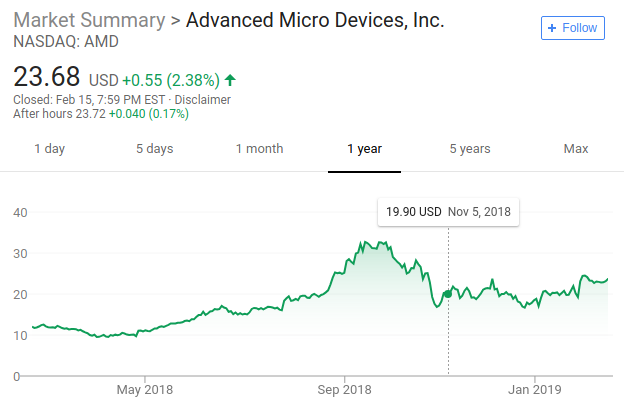
\includegraphics[width=\textwidth]{images/AMDChart.png}
			\caption{A chart of AMD stock prices}
			\label{AMD Chart}
		\end{subfigure}
		\begin{subfigure}[b]{.45\textwidth}
			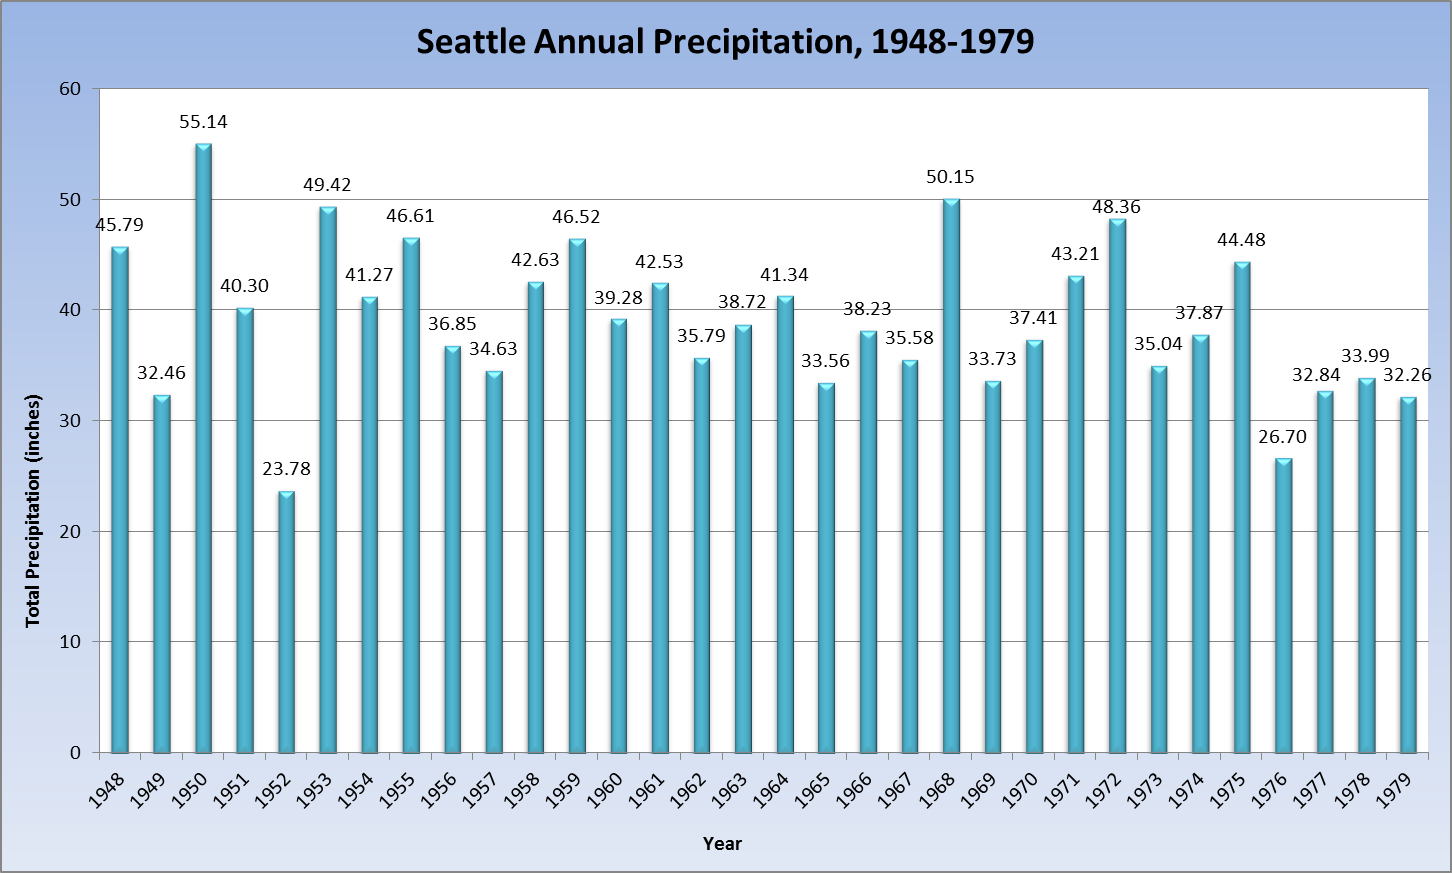
\includegraphics[width=\textwidth]{images/SeattleRainfall.png}
			\caption{Seattle precipitation, 1948-1979}
			\label{AMD Chart}
		\end{subfigure}
		\caption[Examples of Time Series]{Examples of Time Series \footnotemark}
		\label{TimeSeriesExamples}
			
	\end{figure}
\footnotetext{Seattle precipitation image courtesy of Seattle Weather Blog: \href{http://www.seattleweatherblog.com/rain-stats/}{\texttt{http://www.seattleweatherblog.com/rain-stats/}} }
	
	\textcolor{red}{Talk about ARIMA models}
	
	\chapter{Cortical Learning Algorithms}
	
	\section{The Neocortex}
	
	\textcolor{red}{Vernon Mountcastle}
	
	\textcolor{red}{Overview of the neocortex}
	
	\textcolor{red}{Cortical Columns and Pyramidal Neurons}
	
	\begin{figure}[h!]
		\centering
		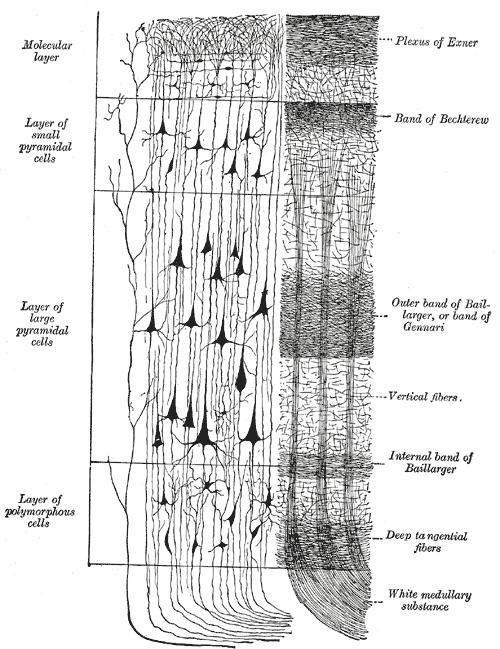
\includegraphics[width=8cm]{images/ColumnOfNeocortex.png}
		\caption{Column of the Neocortex}{Column of the Neocortex\footnotemark}
		\label{CorticalColumn}
	\end{figure}
	\footnotetext{Image courtesy of Wikipedia: \href{https://en.wikipedia.org/wiki/Neocortex}{\texttt{https://en.wikipedia.org/wiki/Neocortex}}}
	
	\section{Sparse Distributed Representations}
	
	Consider the binary representation of the integer 16 versus that of the integer 15. The two numbers are quite similar: they are only 1 apart, so they are as close as two integers can be. Yet their binary representations are [100000] and [011111] respectively. They have no shared ``on'' bits so despite their similarity, their binary representations reflect none at all. In fact, despite being as close as two integers can be (a Euclidean distance of 1), their binary representations have a Hamming distance, the number places in which two codewords differ, of 5, the maximum Hamming distance of two codewords of length 5 \cite{Adams}. 
	
	This means that our encoding does not preserve semantic similarity or a concept of distance between elements which is highly undesirable for an code because if there is some kind of error in the code we could end up decoding something meaning the opposite of what we were trying to convey. As an example, consider $\mathbb{Z}$ from 0 to 31 which is mapped to $GF(2)^{6}$ by their binary representation. The mapping of 31 is [111111] but a single error in transmission can easily lead to [011111] which would be decoded as 15. So a code Hamming distance ($d_{H}$) of one away ($\frac{1}{5}$ of the total metric) lead to an element 16 integers away ($\frac{1}{2}$ of the total metric). We would obviously like to avoid this so that errors in the transmission of our codes are either (1) correctable or (2) lead to a decoding that is as close as possible to our original element.
	
	This is achievable by simply conveying more information in our code. In our binary representation any single error led to another valid codeword (a codeword which decoded to an element of the input/output set) which meant that no errors could be detected or corrected. By expanding our code length, we increase the number of codewords (multiplying by the cardinality of the code alphabet for each character added) meaning that fewer errors will result in other valid codewords and can possibly be detected or corrected. 
	
	A key strategy with Sparse Distributed Representations is to encode semantic similarity, such as with our idea of distance in our motivating example. This helps us achieve our second goal because even if we increase the error-tolerance of our code, there is still some probability of an uncorrectable error and we would like that error to result in a codeword as close to the original codeword as possible. To give you a real world example imagine I am sending instructions to a aircraft and I need to tell it to turn down 7\textdegree~to start its descent. Obviously, an error resulting in 8\textdegree~or 6\textdegree~being interpretted by the pilot are both preferable to 90\textdegree.
	
	To achieve our goal, we employ sparse distributed representations or SDRs. Just as with traditional dense binary representations, we will represent sparse distributed representations as vectors over their code alphabet, in this case GF(2). We call them \textbf{sparse} distributed representations because these vectors typically only have a small proportion of the components as 1. We will use Numenta's notation of letting $w_{\overrightarrow{x}}$ denote the number of components in an SDR $\overrightarrow{x}$ that are 1, so $w_{\overrightarrow{x}} = \norm{x}_{1}$ \cite{Properties}.
	
	Given our definition of distance, we could say that two decodings of sparse distributed representations, $a$ and $b$, are equal if and only if the $d_{H}(a,b) = w_{a} = w_{b}$. This would mean that both vectors would have to have the same dimensionality, same number of on bits, and all on and off bits would have to match. This definition is good for ``equals,'' but suppose we have a single error in transmission or a single component of our distributed system fails, equality would thus fail. In order to be able preserve the ability to subsample and thus to preserve fault tolerance, we therefore need a less stringent definition for decoding SDRs. Numenta refers to this as the $overlap$, which is $$ overlap(\overrightarrow{a}, \overrightarrow{b}) \equiv \overrightarrow{a} \cdot \overrightarrow{b} \equiv \sum_{0}^{n-1} a_{i}b_{i}$$ Thus, we say two SDRs $\overrightarrow{a}$ and $\overrightarrow{b}$ decode to the same element of the input space if and only if $overlap(a,b) \geq \theta$ where $\theta \leq w_{a}$ and $\theta \leq w_{b}$ \cite{Properties}. Denote the function that determines if two sparse distributed representations decode to the same element of the input space using some $\theta$ and $overlap(\overrightarrow{a}, \overrightarrow{b})$, $match_{\theta}(\overrightarrow{a}, \overrightarrow{b})$ and it is a function from SDR$\times$SDR $\longrightarrow$\{true, false\}.
	
	Given a set of sparse distributed representations with the same dimension, $X =\{\overrightarrow{x_{1}}, \overrightarrow{x_{2}}, ...,\overrightarrow{x_{n}}\}$, we can union the vectors using the bitwise OR operation over the $i^{th}$ position of the vectors in the set to produce the $i^{th}$ position of $union(X)$ \cite{Properties}. For example, given [0100] and [0010] the union would be [0110]. We say an SDR $\overrightarrow{y}$ is an element of the union of a set of SDRs, $\overrightarrow{X}$, if and only if $match_{\theta}(\overrightarrow{X},\ \overrightarrow{y})$ \cite{Properties}.
	
	\section{Hierarchical Temporal Memory}
	
	Hierarchical Temporal Memory aims to implement the functions of the neocortex as faithfully as possible, and unsurprisingly uses the same atomic unit of the cell. Modeled after the pyramidal neurons of the neocortex, these cells each take their own inputs and make their own predictions which the layer combines into a cohesive prediction \cite{Whitepaper}. They have three states: active from feed-forward input, active from lateral input (predictive state), and inactive. These first two states correspond to a short burst of action potentials in a neuron, and a slower steady burst of action potentials on a neuron respectively in our own brain.
	
	\begin{figure}[h!]
		\centering
		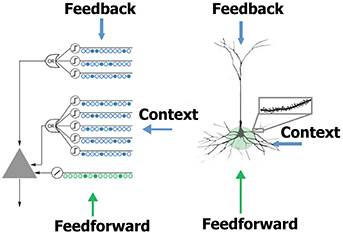
\includegraphics[width=\linewidth]{images/HTMCell.jpg}
		\caption{Pyramidal Neuron vs. Hierarchical Temporal Memory Cell}
		\label{fig:HTMCell}
	\end{figure}

	Just like actual pyramidal neurons, HTM cells also dendrite segments. Each cell has one proximal dendrite segment and a dozen or more distal dendrite segments \cite {Whitepaper}. Proximal dendrites accept feed-forward input and all cells in the same column respond to a similar feed-forward input due to a class of inhibitory cells. On the other hand, distal dendrites receive lateral input from nearby cells and their response is unique on a cell-by-cell basis dependent on the connected synapses on each cells distal dendrites. Figure~\ref{fig:HTMCell} illustrates the similarities between a pyramidal neuron and an HTM cell.
	
	\textcolor{red}{talk about synapses}
	
	\subsection{Encoder}
	
	\subsection{Spatial Pooler}
	
	\subsection{Temporal Pooler}


	\begin{figure}[h!]
		\centering
		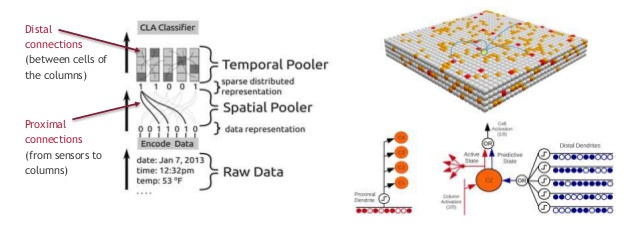
\includegraphics[width=\linewidth]{images/Poolers.jpg}
		\caption{Spatial and Temporal Poolers}
		\label{fig:Poolers}
	\end{figure}

	\subsection{Classifier}
	
	Once the system completes its processing of a time step's input, the system outputs a sparse distributed representation which may have gone through multiple layers and it is important to be able to decode the system's prediction in order for the system to be useful. Hierarchical Temporal Memory currently uses something called an SDR Classifier to decode the predictions of an HTM \cite{Dillon}. At its essence, an SDR Classifier is a single layer, feed forward, neural network \cite{Dillon}.
	
	\begin{figure}[h!]
		\centering
		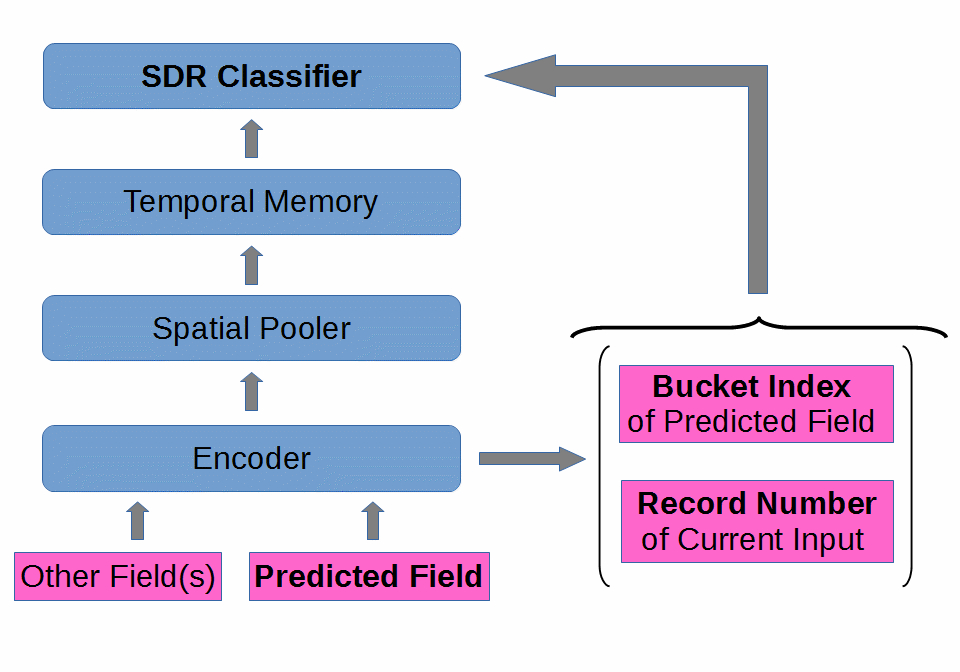
\includegraphics[width=.6\linewidth]{images/SDRClassifier.jpg}
		\caption{SDR Classifier}
		\label{fig 3}
	\end{figure}
	
	SDR Classifiers are able to decode the information HTMs give about predictions $n$ times steps in the future by maintaining a weight matrix \cite{Dillon}. The matrix's weights are adjusted to ``learn'' after each time step to reflect the correct weighting between the output vector at time $t$ and the probability distribution of the input/output space at time $t-n$ \cite{Dillon}. This enables the matrix to reflect relationships between inputs and outputs $n$ time steps apart. To determine the SDR Classifier's interpretation of an output at time $t+n$, the SDR Classifer takes in the HTM's output vector and uses Softmax to determine the most likely decoding \cite{Dillon}. So for each of the $k$ classes in the output space, the certainty that the output vector is referring to it is $$y_{j} = \dfrac{e^{a_{j}}}{\sum_{i=1}^{k} e^{a_{i}}}$$ where $a_{j}$ is the activation level of the $j^{th}$ element of the output space, calculated by multiplying the output vector by the $j^{th}$ column of the weight matrix element wise \cite{Dillon}. 
	
	\chapter{Literature Review}
	
	\section{Sequence Memory for Anomaly Detection and Prediction}
	
	\textcolor{red}{Numenta's work}
	
	\textcolor{red}{partners such as http://numenta.com/htm-for-stocks/ grokstream.com cortical.io}
	
	\textcolor{red}{Masters theses on prediction}
	
	\section{Spatial Data, Sensors, and Motor Response}
	
	\chapter{Experiment Design}
	
	\section{Hardware and Software Specifications}
	
	I utilized the official Python (Python 2.7) implementation of Numenta's cortical learning algorithms, NuPIC\footnote{NuPIC repository: \href{https://github.com/numenta/nupic}{\ttfamily https://github.com/numenta/nupic} } and it's Network API\footnote{Network API docs: \href{http://nupic.docs.numenta.org/stable/api/network/}{\ttfamily http://nupic.docs.numenta.org/stable/api/network/}}. At the time of my work NuPIC was at version 1.05 and I chose to use this version. It should be noted that although much of NuPIC is in Python, many of its computationally intensive algorithms are implemented in C++ using their NuPIC.core repository\footnote{NuPIC.core repository: \href{https://github.com/numenta/nupic.core}{\ttfamily https://github.com/numenta/nupic.core}} and it also relies on a number of external libraries such as \texttt{numpy} and \texttt{pandas}. 
	
	Due to the computationally intensive nature of my research and the limited time available to me, I also heavily relied on parallel processing to run my code in a reasonable time frame. In particular, the \texttt{multiprocessing} package in Python was indispensable to my research, allowing me to speed my code up a factor of up to 28x when running independent tests or swarming.
	
	\begin{table}[h!]
		\centering
		\begin{tabular}{|l|l|}
			\hline
			\multicolumn{2}{|l|}{Dijkstra (Asus Vivobook)} \\ \hline
			CPU     & Intel i5-8250U, 4-Core, 1.60GHz     \\ \hline
			RAM     & 24 GB                                \\ \hline
			OS      & Linux Mint 19 Cinnamon               \\ \hline
			\multicolumn{2}{|l|}{Galois (HP DL380 G7)}     \\ \hline
			CPU     &  2x Intel Xeon X5650, 6-Core, 2.70 GHz       \\ \hline
			RAM     & 192 GB                               \\ \hline
			OS      & Linux Mint 19 Cinnamon               \\ \hline
			\multicolumn{2}{|l|}{Aslan (\textbf{Type})}                         \\ \hline
			CPU&    2x  Intel Xeon E5-2690, 10-Core, 3.00 GHz    \\ \hline
			RAM&    252 GB                                  \\ \hline
			OS&    Gentoo                               \\ \hline
		\end{tabular}
		\caption{Hardware Specifications}
		\label{tab:hardware}
	\end{table}

	On the hardware side of things, the majority of development and testing was conducted on my personal laptop, an Asus Vivobook with some small upgrades (see Table~\ref{tab:hardware} for details). The code was then deployed to my HP DL380 G7 or \textbf{[ASLAN's type]} server which had more cores, more memory, and a higher clock speed allowing me to get faster results. For a synopsis of the hardware specifications, see Table~\ref{tab:hardware}. 
	
	\textcolor{red}{Hardware and language}
	
	\textcolor{red}{Numerical analysis-Epsilon comparisons}
	
	\section{Particle Swarm Optimization}
	
	Introduced in by Russell Eberhart and James Kennedy in their 1995 paper, \textit{A New Optimizer Using Particle Swarm Theory}, Particle Swarm Optimization has changed the way the world optimizes continuous nonlinear functions~\cite{PSOReview}. Swarming is fast and effective for optimization over complex multidimensional search spaces and lends itself well to parallelization due to its multi-agent approach, making it an excellent choice for optimizing parameters in neural networks and is implemented by Numenta for finding optimal parameters.
	
	Usually abbreviated to PSO or \textit{swarming}, it draws inspiration from bird flocks and schools of fish~\cite{Eberhart}. The concept is quite simple: it simulates particles on parameter space and at each time-step every particle evaluates fitness as a function of its location in parameter space, then moves towards some linear combination of its personal best and the overall best score among the particles using weights representing a cognitive constant or individuality (denoted $c$) and a social constant (denoted $s$).
	
	\begin{figure}[h!]
		\centering
		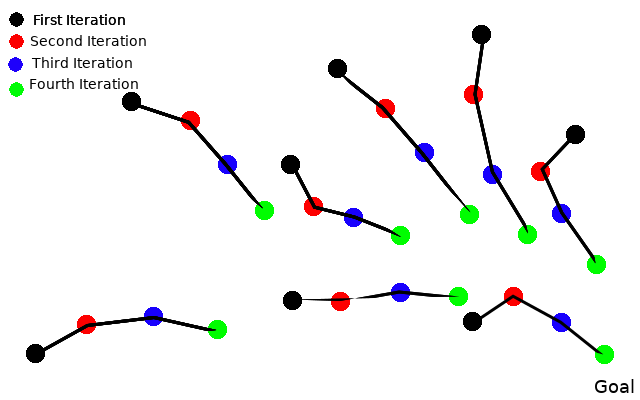
\includegraphics[width=.7\linewidth]{images/PSOVisual.png}
		\caption{Visualization of the PSO Algorithm}
		\label{fig:PSOVisual}
	\end{figure}
	
	The algorithm begins by initializing all particles with a random coordinate in the parameter space and a random velocity. Then at each time step, it calculates its fitness based on the function being optimized and the parameters associated with its position in parameter space. If this fitness is the best the particle has achieved, it is recorded as its personal best, denoted \texttt{pbest} and the particle with the best fitness is chosen as global best, denoted \texttt{gbest}. We then update the velocity and particle position of each particle in our swarm using the equations described in Equation~\eqref{eqn:psoupdate} where $v_{t}$ is the velocity of a particle at time step $t$, $p_{t}$ is the position of a particle at time step $t$, and $\beta_{1}, \beta_{2}$ are uniformly distributed random variables with $\max(\beta)$ being a parameter of the algorithm~\cite{PSOReview}.
	
	\begin{align}
	\label{eqn:psoupdate}
	\begin{split}
	v_{t+1} &= v_{t}+c\times \beta_{1} \times (\text{pbest}-p_{t})+s\times \beta_{2} \times (\text{gbest}-p_{t}), \\
	p_{t+1} &= p_{t} + v_{t+1} .
	\end{split}
	\end{align}
	
	\textcolor{red}{Wrote wrapper and swarming utility}
	
	\textcolor{red}{LOTS of swarming}
	
	\chapter{Results and Discussion}
	
	\chapter{Further Work}
	
	
	
	\blankpage
	\addcontentsline{toc}{chapter}{References}
	\bibliographystyle{siam}     % Siam and Ieeetr bibliographic styles treat titles of articles in journals or collections correctly
	\nocite{*}  % List ALL references in your references, not just the ones cited in the text.
	% This scheme automatically alphabetizes the Bibliography.
	\bibliography{Bibliography}{}
	
	\appendices
	\addcontentsline{toc}{chapter}{Appendix}
	
\end{document}
